% This file was created with tikzplotlib v0.10.1.
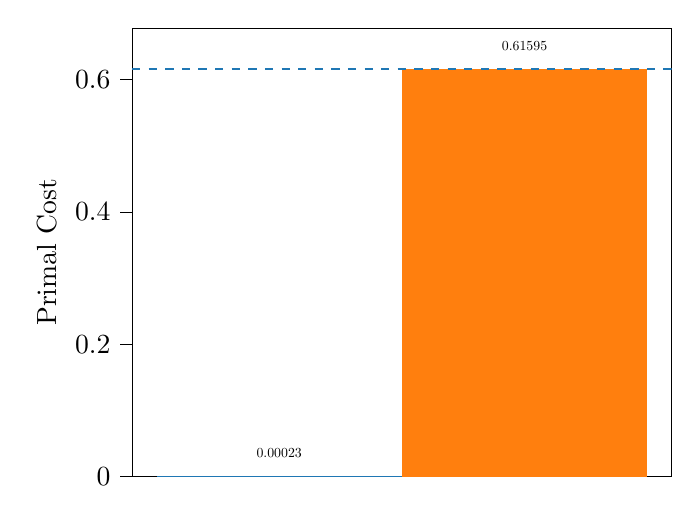
\begin{tikzpicture}

\definecolor{darkgray176}{RGB}{176,176,176}
\definecolor{darkorange25512714}{RGB}{255,127,14}
\definecolor{lightgray204}{RGB}{204,204,204}
\definecolor{steelblue31119180}{RGB}{31,119,180}

\begin{axis}[
legend cell align={left},
legend style={
  fill opacity=0.8,
  draw opacity=1,
  text opacity=1,
  at={(1,0.5)},
  anchor=west,
  draw=lightgray204
},
scaled x ticks=manual:{}{\pgfmathparse{#1}},
tick align=outside,
x grid style={darkgray176},
xmajorticks=false,
xmin=-0.44, xmax=0.44,
xtick style={color=black},
xticklabels={},
y grid style={darkgray176},
ylabel={Primal Cost},
ymin=0, ymax=0.677542387388622,
ytick pos=left,
ytick style={color=black}
]
\draw[draw=none,fill=steelblue31119180] (axis cs:-0.4,0) rectangle (axis cs:0,0.000231313597978408);
\draw[draw=none,fill=darkorange25512714] (axis cs:-2.77555756156289e-17,0) rectangle (axis cs:0.4,0.615947705947281);
\addplot [semithick, steelblue31119180, dashed, forget plot]
table {%
-0.44 0.615947624898747
0.44 0.615947624898747
};
\draw (axis cs:-0.2,0.000231313597978408) ++(0pt,5pt) node[
  scale=0.5,
  anchor=south,
  text=black,
  rotate=0.0
]{0.00023};
\draw (axis cs:0.2,0.615947705947281) ++(0pt,5pt) node[
  scale=0.5,
  anchor=south,
  text=black,
  rotate=0.0
]{0.61595};
\end{axis}

\end{tikzpicture}
